\documentclass[12pt,letterpaper]{article}
\usepackage[utf8]{inputenc}
\usepackage[spanish]{babel}
\usepackage{graphicx}
\usepackage[left=2cm,right=2cm,top=2cm,bottom=2cm]{geometry}
\usepackage{graphicx} % figuras
% \usepackage{subfigure} % subfiguras
\usepackage{float} % para usar [H]
\usepackage{amsmath}
%\usepackage{txfonts}
\usepackage{stackrel} 
\usepackage{multirow}
\usepackage{enumerate} % enumerados
\renewcommand{\labelitemi}{$-$}
\renewcommand{\labelitemii}{$\cdot$}
% \author{}
% \title{Caratula}
\begin{document}

% Fancy Header and Footer
% \usepackage{fancyhdr}
% \pagestyle{fancy}
% \cfoot{}
% \rfoot{\thepage}
%

% \usepackage[hidelinks]{hyperref} % CREA HYPERVINCULOS EN INDICE

% \author{}
\title{Caratula}

\begin{titlepage}
\begin{center}
\large{UNIVERSIDAD PRIVADA DE TACNA}\\
\vspace*{-0.025in}
\begin{figure}[htb]
\begin{center}

\includegraphics[width=7cm]{./images/logo}
\end{center}
\end{figure}
\vspace*{0.15in}
INGENIERIA DE SISTEMAS  \\

\vspace*{0.3in}
\begin{large}
\textbf{TITULO:} \\
\end{large}

\vspace*{0.1in}
\begin{Large}
\textbf{Informe de Laboratorio 01} \\

\end{Large}

\vspace*{0.3in}
\begin{Large}
\textbf{CURSO:} \\
\end{Large}

\vspace*{0.1in}
\begin{large}
Calidad y Pruebas de Software\\
\end{large}

\vspace*{0.3in}
\begin{Large}
\textbf{DOCENTE:} \\
\end{Large}

\vspace*{0.1in}
\begin{large}
 Ing. Patrick Cuadros Quiroga\\
\end{large}

\vspace*{0.4in}
\vspace*{0.1in}
\begin{large}
\textbf{INTEGRANTES:} \\
\begin{flushleft}
Katerin Almendra Merino Quispe \hfill	(2018060918)\\

\centering  %CENTRA UN TEXTO
\vspace*{0.9in}
\begin{large}
Tacna
\end{large}

\end{flushleft}
\end{large}
\end{center}

\end{titlepage}


\tableofcontents % INDICE
\thispagestyle{empty} % INDICE SIN NUMERO
\newpage
\setcounter{page}{1} % REINICIAR CONTADOR DE PAGINAS DESPUES DEL INDICE


\section{Paso 1:Descargar SonarQube} 
docker pull sonarqube
\begin{center}
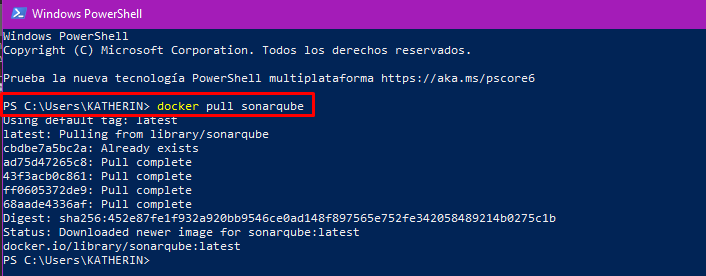
\includegraphics[width=\columnwidth]{images/1}\newline
\end{center}
\section{Paso 2: Ejecutar una instancia de SonarQube } 
\begin{itemize}
    \item docker run -d --name sonarqube -p 9000:9000 sonarqube
\end{itemize}
\begin{center}
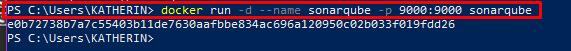
\includegraphics[width=\columnwidth]{images/2}\newline
\end{center}
\section{Paso 3: Ingresar al portal con las credenciales } 
\begin{itemize}
    \item http://localhost:9000/
    \item 192.168.99.100:9000
    \item user: admin
    \item pass:admin
\end{itemize}
\begin{center}
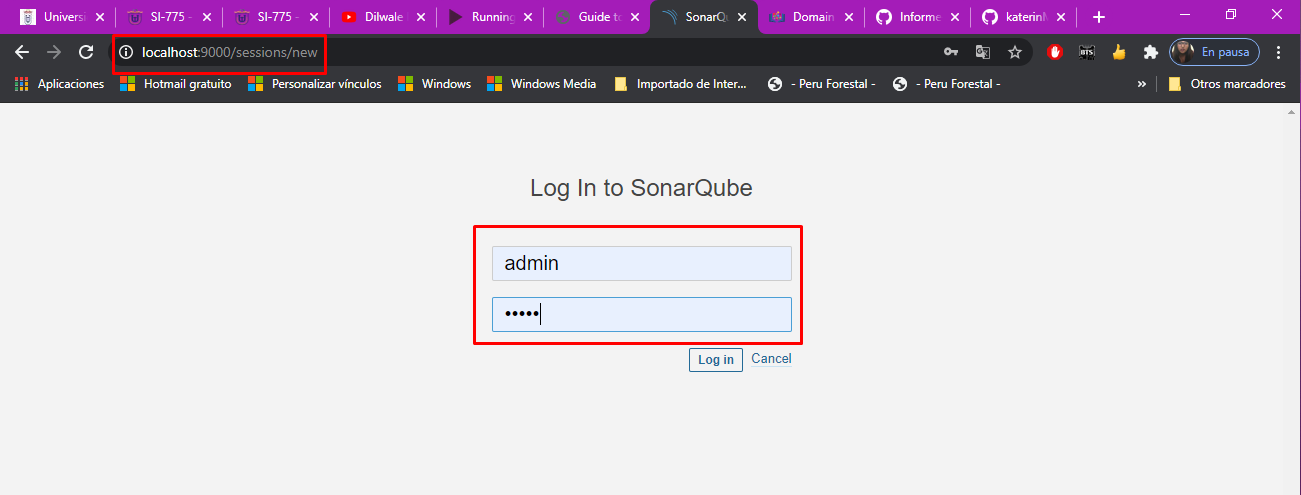
\includegraphics[width=\columnwidth]{images/3}\newline
\end{center}
\section{Paso 4: Crear una nueva aplicación con el nombre aplicacionNetCore } 
\begin{center}
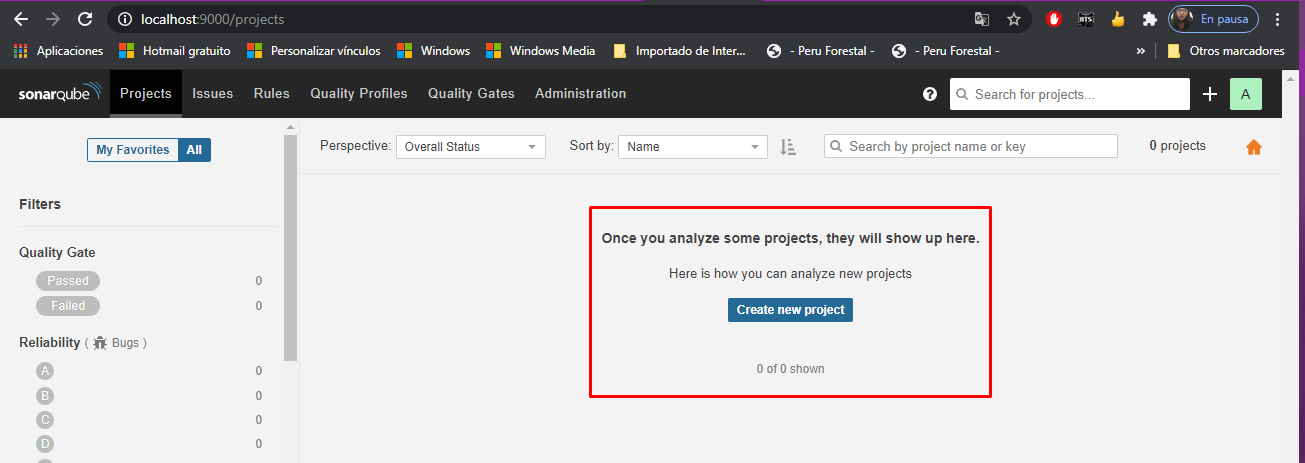
\includegraphics[width=\columnwidth]{images/4}\newline
\end{center}
\section{Paso 5: Generar el token de la nueva aplicación aplicacionNetCore, debera devolver algo similar a 8a15d2a89c8636f15eb32ebee0993b8d16bff94e } 
\begin{center}
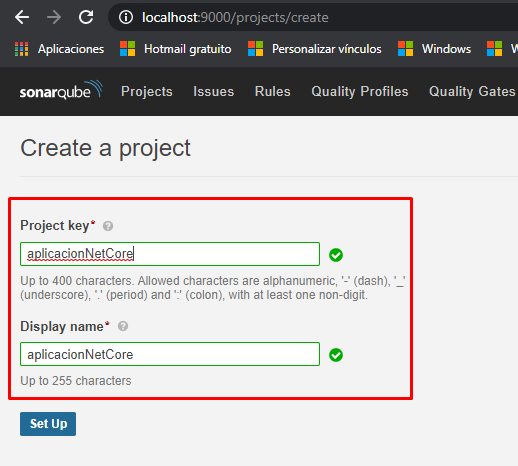
\includegraphics[width=\columnwidth]{images/5}\newline
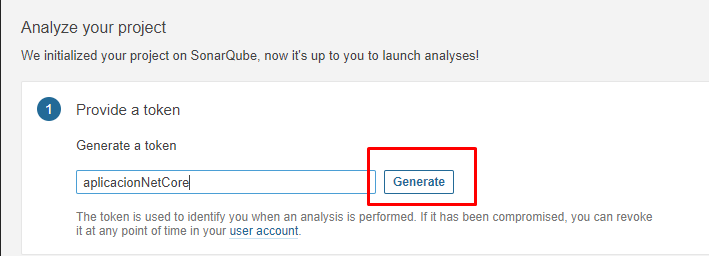
\includegraphics[width=\columnwidth]{images/6}\newline
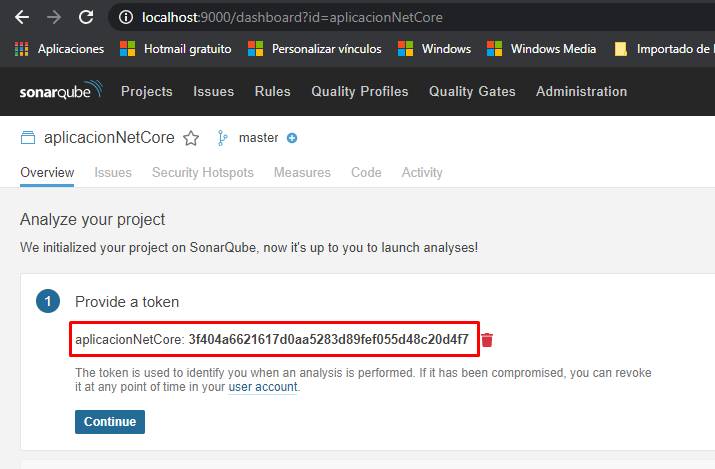
\includegraphics[width=\columnwidth]{images/7}\newline
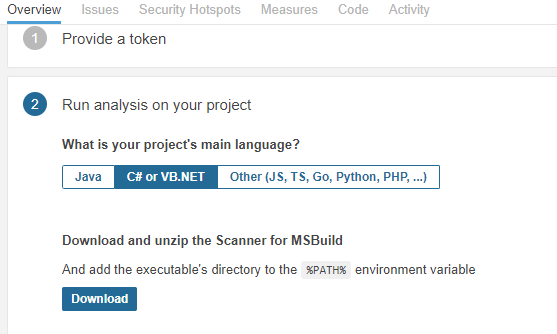
\includegraphics[width=\columnwidth]{images/8}\newline
\end{center}
\section{Decargar Net Core e instalar} 

\begin{itemize}
    \item  https://dotnet.microsoft.com/download/dotnet-core/thank-you/sdk-3.1.300-windows-x64-installer
\end{itemize}
\begin{center}
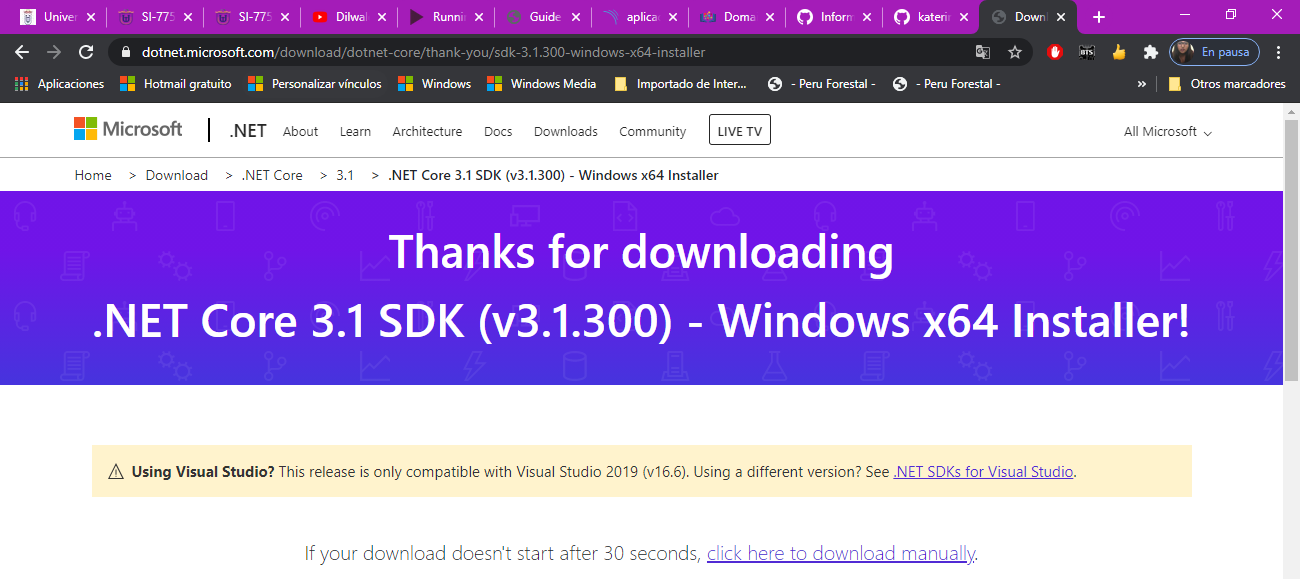
\includegraphics[width=\columnwidth]{images/18}\newline
\end{center}

\section{En un terminal ejecutar e instalar sonar-scanner} 
\begin{itemize}
    \item  dotnet tool install --global dotnet-sonarscanner
\end{itemize}
\begin{center}
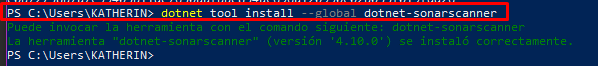
\includegraphics[width=\columnwidth]{images/10}\newline
\end{center}
\section{En un terminal, acceder a una ruta donde creara una nueva aplicacion } 
\begin{itemize}
    \item dotnet new sln -o aplicacionNetCore 
    \item cd aplicacionNetCore 
    \item dotnet new console
    \item dotnet sln aplicacionNetCore.sln add aplicacionNetCore.csproj 
\end{itemize}
\begin{center}
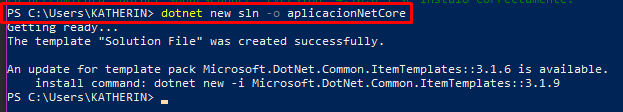
\includegraphics[width=\columnwidth]{images/11}\newline
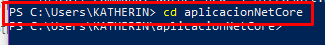
\includegraphics[width=\columnwidth]{images/12}\newline
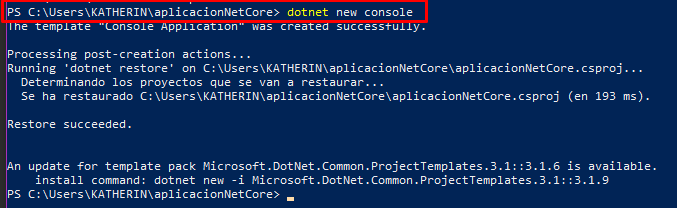
\includegraphics[width=\columnwidth]{images/19}\newline
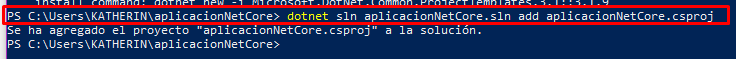
\includegraphics[width=\columnwidth]{images/20}\newline

\end{center}
\section{ En el mismo terminal, iniciar la sesión de revisión de sonarqube } 
\begin{itemize}
    \item dotnet SonarScanner begin /k:"aplicacionNetCore" /d:sonar.host.url="http://localhost:9000" /d:sonar.login="e7e2acdf4d6e5469cd486b29068f0b5ab9d8ad2e"
\end{itemize}
\begin{center}
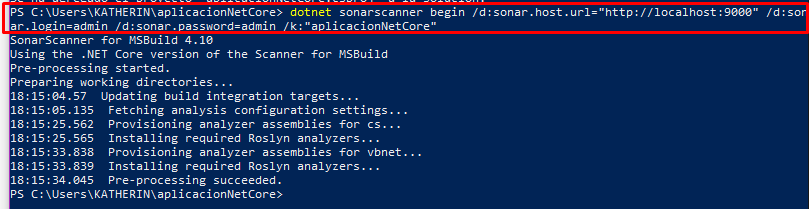
\includegraphics[width=\columnwidth]{images/13}\newline
\end{center}
\section{ Compilar la aplicación } 
\begin{itemize}
    \item dotnet build
\end{itemize}
\begin{center}
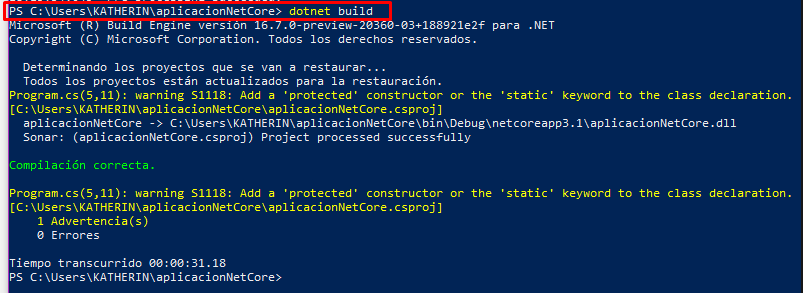
\includegraphics[width=\columnwidth]{images/14}\newline
\end{center}
\section{ Cerramos la sesión } 
\begin{itemize}
    \item dotnet SonarScanner end /d:sonar.login="e7e2acdf4d6e5469cd486b29068f0b5ab9d8ad2e"
\end{itemize}
\begin{center}
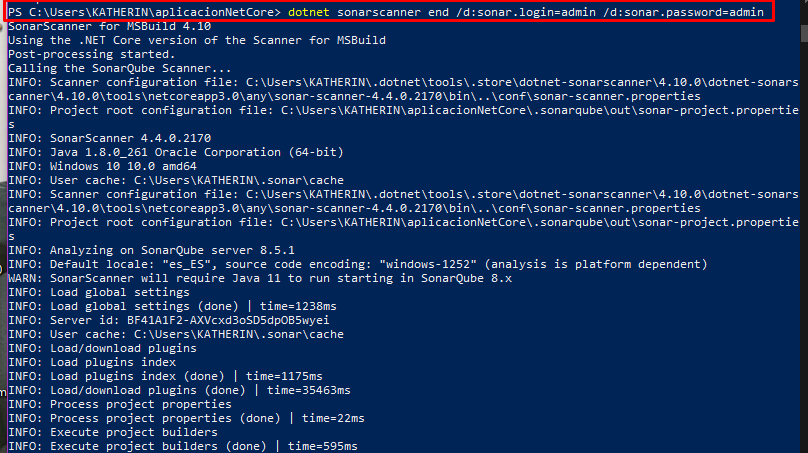
\includegraphics[width=\columnwidth]{images/15}\newline
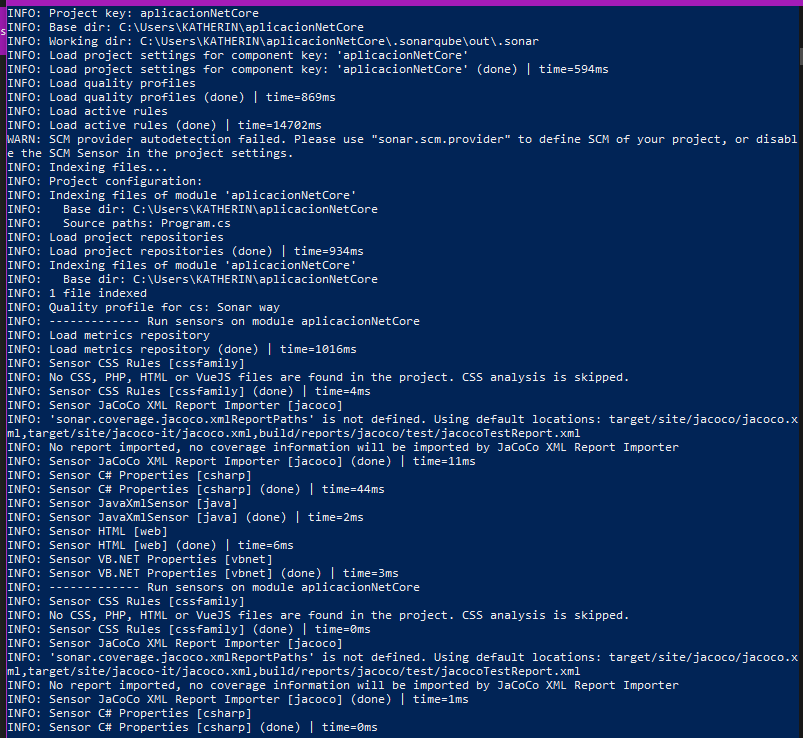
\includegraphics[width=\columnwidth]{images/16}\newline
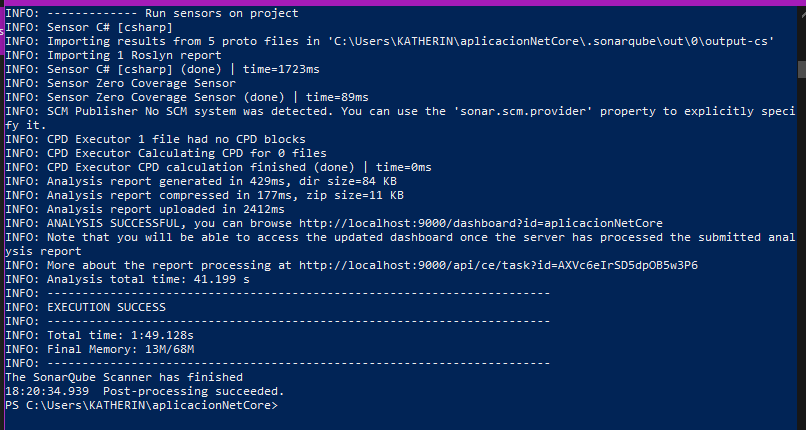
\includegraphics[width=\columnwidth]{images/21}\newline

\end{center}

\section{ Resultado Final }
\begin{itemize}
    \item Asi queda nuestro proyecto final.
    \begin{center}

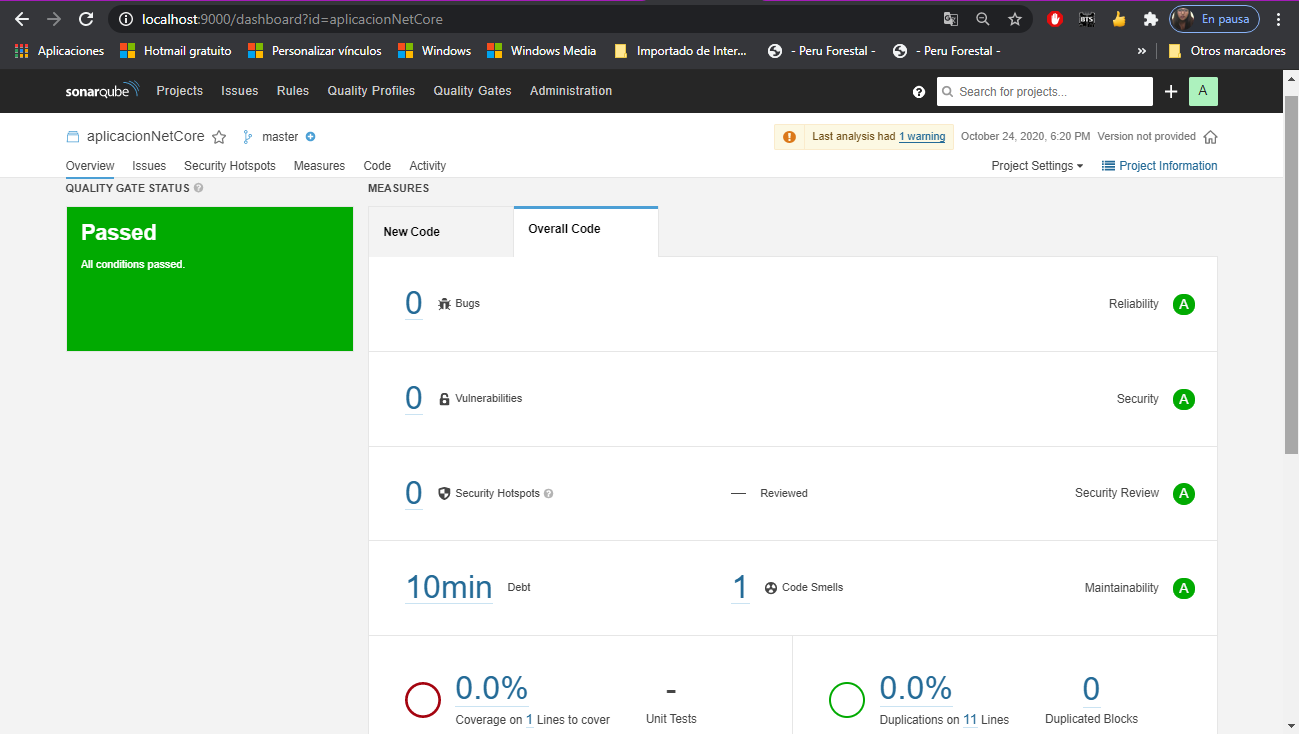
\includegraphics[width=\columnwidth]{images/17}\newline
\end{center}
\end{itemize}

\end{document}